\documentclass[hyperref={pdfpagelabels=false},table,9pt,compress]{beamer}
% File Name: SetUp.tex
% Function: Make main settings of the document.


%%%%%%%%%%%%%%%%%%%%%%%%%%% BEGIN-Theme-settings %%%%%%%%%%%%%%%%%%%%%%%%%%
%%%%% http://www.hartwork.org/beamer-theme-matrix/
\usetheme{default} % Set the theme of the beamer.
%\usetheme{Frankfurt}                     %% Geovani style
%\setbeamercolor{alerted text}{fg=blue}   %% Geovani style
% W/o������:default, boxes, Bergen, Madrid, Pittsburgh, Rochester
% ���������:Antibes, JuanLesPins, Montpellier��
% ��Ŀ¼(TOC)�IJ�ߵ�����: Berkeley, PaloAlto, Goettingen, Marburg, Hannover��
% ��΢��frame������:Berlin, Ilmenau, Dresden, Darmstadt, Frankfurt, Singapore, Szeged��
% ����С�ڱ���: Copenhagen, Luebeck, Malmoe, Warsaw��
%\usecolortheme{default}  % Outer color themes. Alternatives: whale, seahorse, dolphin. default, beaver
\usecolortheme{orchid}  % Inner color themes. Alternatives: lily, orchid.
\useinnertheme[shadow]{rounded}
\usefonttheme{structurebold} % Font themes. Alternatives:  default, serif, structurebold, structureitalicserif, structuresmallcapsserif
\setbeamertemplate{frametitle}
{   \begin{center}
        \insertframetitle
    \end{center}
}
\setbeamertemplate{itemize items}[default] % Alternatives: default/triangle, circle, square, ball
\setbeamertemplate{enumerate items}[default] % Alternatives: default, circle, square, ball
\setbeamertemplate{navigation symbols}{}
\setbeamertemplate{footline}[frame number]
%\setbeamertemplate{footline}{%
%  \leavevmode%
%  \hbox{%
%    \begin{beamercolorbox}[wd=.333333\paperwidth,ht=2.25ex,dp=1ex,center]{author in head/foot}%
%      \usebeamerfont{author in head/foot}\insertshortauthor~(\insertshortinstitute)
%    \end{beamercolorbox}%
%    \begin{beamercolorbox}[wd=.333333\paperwidth,ht=2.25ex,dp=1ex,center]{title in head/foot}%
%      \usebeamerfont{title in head/foot}\insertshorttitle
%    \end{beamercolorbox}%
%    \begin{beamercolorbox}[wd=.333333\paperwidth,ht=2.25ex,dp=1ex,right]{date in head/foot}%
%      \usebeamerfont{date in head/foot}\insertshortdate{}\hspace*{2em}
%      \insertframenumber{} / \inserttotalframenumber \hspace*{2ex}
%    \end{beamercolorbox}
%    }%
%  \vskip0pt%
%}
%%%%%%%%%%%%%%%%%%%%%%%%%%%% END-Theme-settings %%%%%%%%%%%%%%%%%%%%%%%%%%%


%%%%%%%%%%%%%%%%%%%%%%%%%%%%%% BEGIN-Packages %%%%%%%%%%%%%%%%%%%%%%%%%%%%%
\usepackage{amsmath,amssymb,amsfonts}
\usepackage{mathrsfs}
\usepackage{color,xcolor}
\usepackage{graphicx,subfigure}
\usepackage{clock} % Use this package to insert a clock in the beamer.
\usepackage{textcomp}
\usepackage[T1]{fontenc}
\usepackage{verbatim}
\usepackage{moreverb}
\usepackage{multirow,multicol}
%\usepackage{url}
%\usepackage[colorlinks,linkcolor=blue,citecolor=blue,urlcolor=blue]{hyperref}%[colorlinks,linkcolor=blue,citecolor=blue,urlcolor=blue]
\usepackage{CJK}
%%%%%%%%%%%%%%%%%%%%%%%%%%%%%%%% END-Packages %%%%%%%%%%%%%%%%%%%%%%%%%%%%%


% \setbeamertemplate{navigation symbols}{} % Disable the buttons at the bottom.

\graphicspath{{Figures/}} % Set the directory where figures are saved.

%\AtBeginSection{
%  \begin{frame}{Outline}
%    \tableofcontents[currentsection,hideallsubsections]
%  \end{frame}
%}
%\AtBeginSubsection{
%  \begin{frame}{Outline}
%    \tableofcontents[currentsection,currentsubsection]
%  \end{frame}
%}
\AtBeginSection{
  \begin{frame}{Outline}
  \large{
  \tableofcontents[sections={\thesection}]  }
  \end{frame}
}

%%%%%%%%%%%%%%%%%%%% BEGIN-Theorem-like Environments %%%%%%%%%%%%%%%%%%%%%
\newtheorem{mybox}{}
\newtheorem{Con}{Conjecture}[section]
\newtheorem{Thm}{Theorem}[section]
\newtheorem{Prop}{Proposition}[Thm]
% show fig and table number
\setbeamertemplate{caption}[numbered]
% show theorems and example number
\setbeamertemplate{theorems}[numbered]
%%%%%%%%%%%%%%%%%%%%% END-Theorem-like Environments %%%%%%%%%%%%%%%%%%%%%%


%%%%%%%%%%%%%%%%%%%%%%%%%% BEGIN-New Commands %%%%%%%%%%%%%%%%%%%%%%%%%%%%
\newcommand{\email}[1]{Email: \href{mailto: #1}{\tt {\color{blue}#1}}}
\newcommand{\red}{\color{red}}
\newcommand{\blue}{\color{blue}}
\newcommand{\brown}{\color{brown}}
\newcommand{\orange}{\color{orange}}
\newcommand{\yellow}{\color{yellow}}
\newcommand{\Real}{\mathbb{R}}
\newcommand{\Tran}[1]{#1^\mathrm{T}}
\newcommand{\st}{\textnormal{s.t.}}
\newcommand{\dist}{\textnormal{dist}}
\newcommand{\bc}{\begin{center}}
\newcommand{\ec}{\end{center}}
\newcommand{\tbf}{\textbf}
\newcommand{\be}{\begin{equation}}
\newcommand{\ee}{\end{equation}}
\newcommand{\ba}{\begin{array}}
\newcommand{\ea}{\end{array}}
\newcommand{\btab}{\begin{table}\begin{tabular}}
\newcommand{\etab}{\end{tabular}\end{table}}
\newcommand{\nn}{\nonumber}
\newcommand{\xn}{x_1,x_2,\ldots,x_n}
\newcommand{\framee}[2]{\frame{\frametitle{#1} #2}}
\newcommand{\reff}[1]{(\ref{#1})} % ������
\newcommand{\inner}[2]{\left\langle#1,#2\right\rangle}

%\renewcommand{\baselinestretch}{1.3}
% Ĭ��������룬������ó����˶���
\renewcommand{\raggedright}{\leftskip=0pt \rightskip=0pt plus 0cm}
\raggedright
%\large
% define Roman numbers
\makeatletter
\newcommand{\rmnum}[1]{\romannumeral #1}
\newcommand{\Rmnum}[1]{\expandafter\@slowromancap\romannumeral #1@}
\makeatother
%%%%%%%%%%%%%%%%%%%%%%%%%%%% END-New Commands %%%%%%%%%%%%%%%%%%%%%%%%%%%%

\usepackage[linesnumbered,ruled,vlined]{algorithm2e}

\begin{document}
\begin{CJK*}{GBK}{kai}

\title[distance geometry]{\textsc{A New Error Function and Its Application in Distance Geometry Problem}}
\author[Zhenli SHENG]{Zhenli Sheng (ʢ����)\\email: {\blue szl@lsec.cc.ac.cn}}
% \institute{Institute of Computational Mathematics and Scientific/Engineering Computing}
\institute[ICMSEC, CAS]{Institute of Computational Mathematics and Scientific/Engineering Computing,\\Chinese Academy of Sciences}
\date[]{joint work with {\blue Prof. Ya-xiang Yuan} \\\textrm{} \\January 8, 2013\\ seminar talk}
\frame{
\titlepage
}

% File Name: ThankYou.tex
% Function: Insert an Outline page.


%\section*{\textsc{Outline}}
%\begin{frame}
%\frametitle{\textsc{Outline}}
%\end{frame}

\begin{frame}
\frametitle{\textsc{Outline}}
\tableofcontents%[pausesections]
\end{frame}


\section{Problem introduction}
\frame{
\frametitle{the Problem}
%\begin{block}{Molecular Conformation (Protein Structure Determination)}
%Given some interatomic distances, realize the structure of the protein.
%\end{block}

\begin{block}{Distance Geometry Problem (DGP)}
For a graph $G=(V,E)$, given a distance matrix $D$ ($L$ and $U$, respectively) on $E$ and an integer $d$, find $x_1,x_2,\ldots,x_n \in \Real^d$, such that
\be \|x_{i}-x_{j}\|=d_{ij},\quad (i,j) \in E. \ee
or
\be l_{ij}\leq \|x_i-x_j\|\leq u_{ij},\quad (i,j) \in E. \ee
\end{block}

\vskip3mm

\begin{itemize}
  \item NP-hard in general
    \begin{itemize}
      \item polynomial-time solvable instances: K-trilateration graph %    (still challenging)
    \end{itemize}
  \item Applications: protein structure determination, sensor network localization, graph drawing, multidimensional scaling, etc
      \vskip-3mm
      \begin{figure}
        \centering
        \subfigure{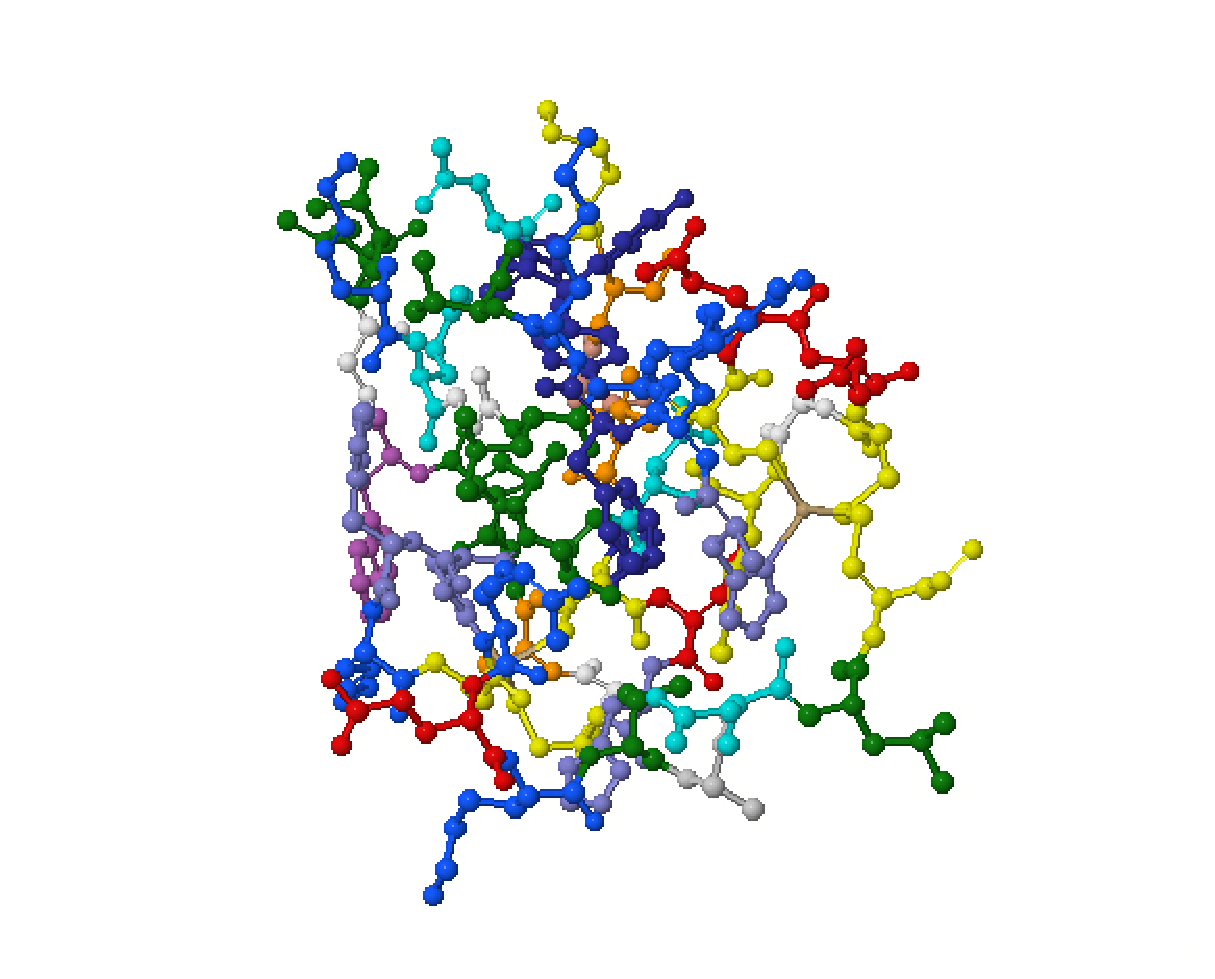
\includegraphics[width=0.21\textwidth]{1PTQ.eps}}\hspace{5mm}
        \subfigure{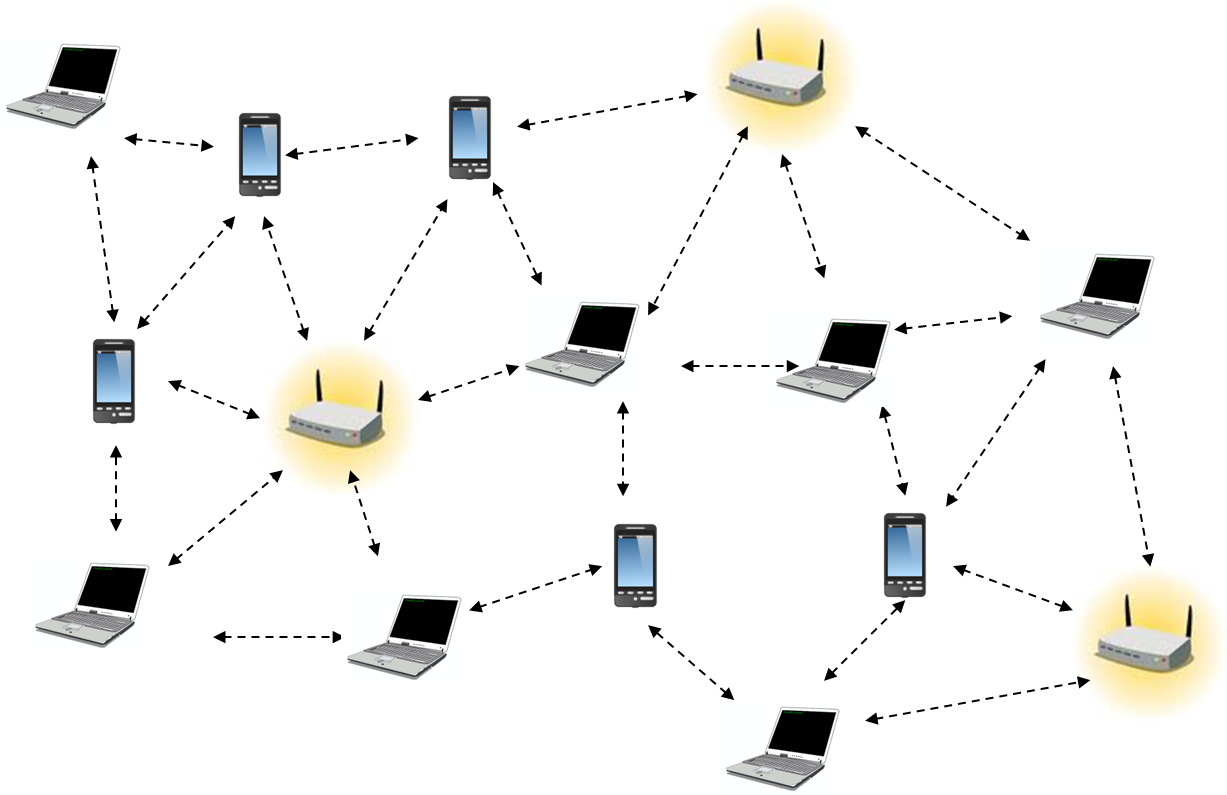
\includegraphics[width=0.2\textwidth]{adhoc.eps}}\hspace{5mm}
        \subfigure{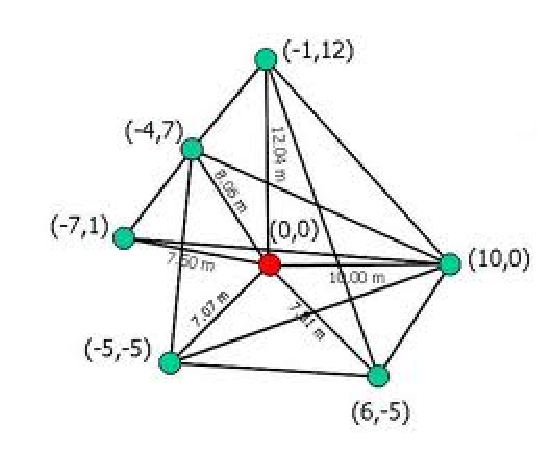
\includegraphics[width=0.2\textwidth]{GraphRealization.eps}}
      \end{figure}
  \item In most instances, distances are \textbf{local}, \textbf{sparse} and \textbf{noisy}.
\end{itemize}
}
%
%\framee{Related Applications/Problems}{
%Some closely related applications/problems:
%\begin{itemize}
%  \item Sensor network localization
%    \begin{itemize}
%        \item $d=2$, anchors
%    \end{itemize}
%  \item Protein structure determination (molecular conformation)
%    \begin{itemize}
%        \item $d=3$, no anchors
%    \end{itemize}
%  \item Graph drawing
%%  \item Dimensionality reduction
%%    \begin{itemize}
%%      \item $d$ unknown, "distances" need be constructed
%%    \end{itemize}
%  \item Euclidean matrix completion
%\end{itemize}
%}

%\framee{}{
%\begin{figure}
%  \centering
%  \subfigure{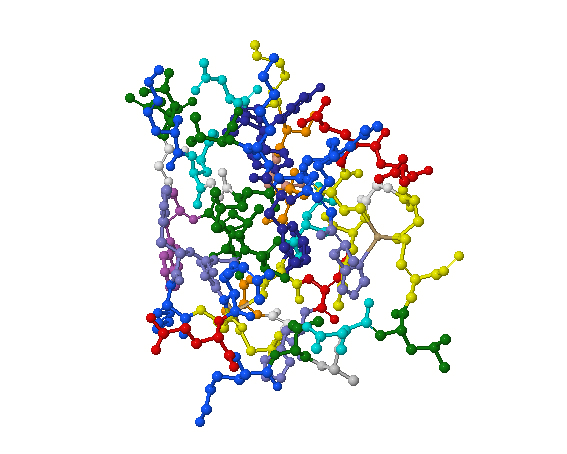
\includegraphics[width=0.45\textwidth]{1PTQ.jpg}}
%  \subfigure{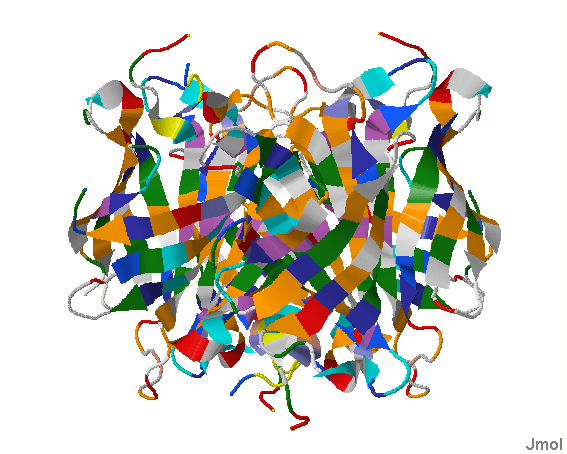
\includegraphics[width=0.45\textwidth]{1HQQ.jpg}}
%  \subfigure{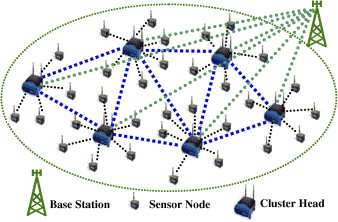
\includegraphics[width=0.45\textwidth]{sensor2.jpg}}
%  \subfigure{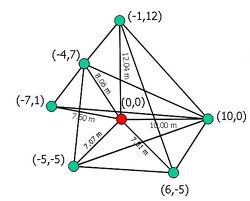
\includegraphics[width=0.45\textwidth]{GraphRealization.jpg}}
%\end{figure}
%}

\framee{Solution Methods}{
\begin{itemize}
  \item Matrix Decomposition Method \paper{Blumenthal 1953, Torgerson  1958}
  \item The Embedding Algorithm \paper{Crippen-Havel 1988}
  \item Global Smoothing Algorithm \paper{Mor$\acute{e}$-Wu 1997}
  \item Geometric Buildup Method \paper{Dong-Wu 2002, Sit-Wu-Yuan 2009, Sheng-Yuan 2014}
  \item SDP Relaxation Method \paper{Biswas-Toh-Ye 2007}
  \item Nearest Euclidean Distance Matrix \paper{Qi-Yuan 2013}
  \item The Branch-and-Prune Algorithm \paper{Liberti-Lavor-Maculan-Mucherino 2014}
  \item and so on ...
\end{itemize}
}

\framee{Models: error functions}{
The problem is usually modeled as an unconstrained \textbf{global} optimization problem.
\vskip-1mm
\begin{itemize}
  \item Stress function
  \be Stress(\xn) = \sum_{(i,j)\in E} \omega_{ij} (\|x_i-x_j\|-d_{ij})^{2} \ee
  \vskip-3mm
  \begin{itemize}
    \item $\omega_{ij}$ specify the degree of confidence or simply weights to balance all the terms
    \item $\omega_{ij}=1$: raw stress function
    \item $\omega_{ij}=1/d_{ij}^2$: relative errors
  \end{itemize}
  \item Smoothed Stress function
  \be SStress(\xn) = \sum_{(i,j)\in E} \omega_{ij}(\|x_i-x_j\|^2-d_{ij}^2)^{2}\ee
  \item Absolute Error function
  \be AbsErr(\xn) = \sum_{(i,j)\in E} \omega_{ij}\left|\|x_i-x_j\|^2-d_{ij}^2
  \right| \ee
  \item our proposed function
  \be f(\xn) = \sum_{(i,j)\in E} \omega_{ij}h(\frac{\|x_i-x_j\|}{d_{ij}}), ~~~h(x) = \left\{ \begin{array}{ll}
                  \frac{1}{2}(x-1)^{2} & x\geq 1 \\
                  x-1-ln(x)          & x<1
                \end{array}   \right. \ee
\end{itemize}
}

%\framee{Geometric Buildup Method}{
%Key ideas:\\
%\begin{itemize}
%  \item Observation: a point in $\mathbb{R}^d$ can be uniquely determined by $d+1$ distances to the determined points (not in a $d-1$ dimensional hyperplane)
%  \item Determine the points one by one
%\end{itemize}
%\vskip2mm
%%\begin{algorithm}[H]
%%%\SetKwInOut{Init}{Initialization}
%%%\vspace{0.3cm}
%%\KwIn{A symmetric distance matrix $D$ to specify part of the pairwise distances}
%%\KwOut{the set of determined points and the corresponding coordinates $X$}
%%\vskip3mm
%%Determine four initial points \\
%%\While{some undetermined points can be determined}{
%%Choose point $j$ which has at least four distances to the determined points, \\
%%Determine $X_j$ by solve linear/nonlinear least square.
%%}
%%\caption{Geometric Buildup Method for sparse noisy anchor-free DGP}
%%\end{algorithm}
%
%\begin{algorithm}[H]
%\KwIn{A symmetric distance matrix $D$ to specify part of the pairwise distances}
%\KwOut{the set of determined points and the corresponding coordinates $X$}
%%\vskip1mm
%Find four points that are not in the same plane
%
%Determined the positions of the four points with the distance among them
%
%Repeat:\\
%\For{each of the undetermined points}{
%\If{the point has $l~(l\geq 4)$ distances to determined points that are not in the same plane}{Determine the position(s) by linear (nonlinear) least square}
%}
%If no more points can be determined in the loop, stop.
%\caption{Geometric Buildup Method for sparse noisy anchor-free DGP}
%\end{algorithm}
%}


\framee{Motivation: a short story}{
When I was an undergraduate student, I read the papers about Geometric Buildup Method and wrote {\tt MATLAB} code to implement it, I found that
\bc \textbf{Error Accumulation is a DEVIL! }\ec
I came up with two ideas:
\begin{itemize}
  \item design strategies to prevent error accumulation (linear/nonlinear least square)
  \item divide and conquer (Laplacian matrix)
\end{itemize}

\begin{figure}
  \centering
  \subfigure{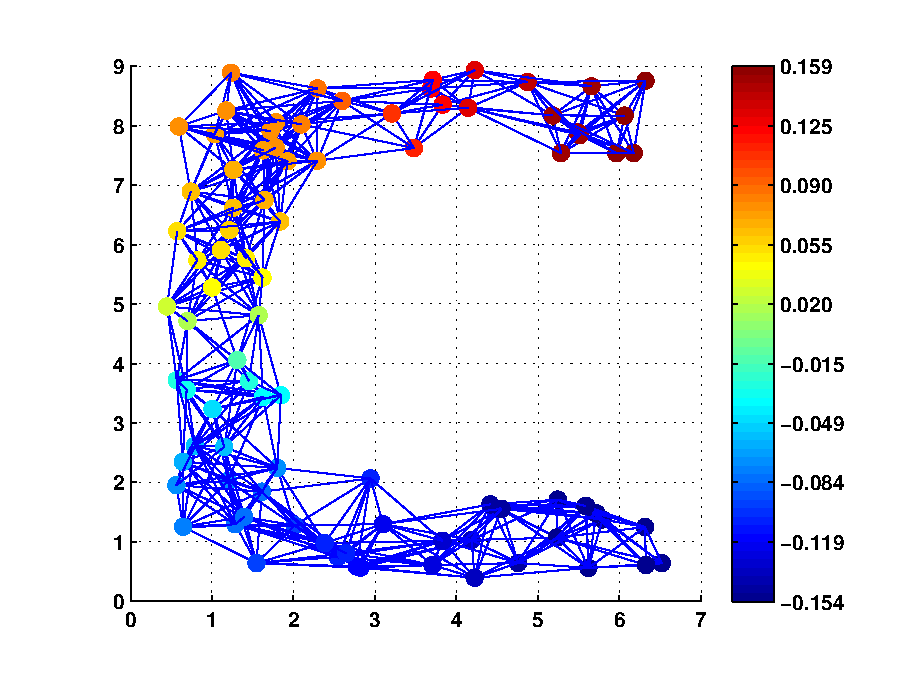
\includegraphics[width=0.45\textwidth]{eig_one.eps}}
  \subfigure{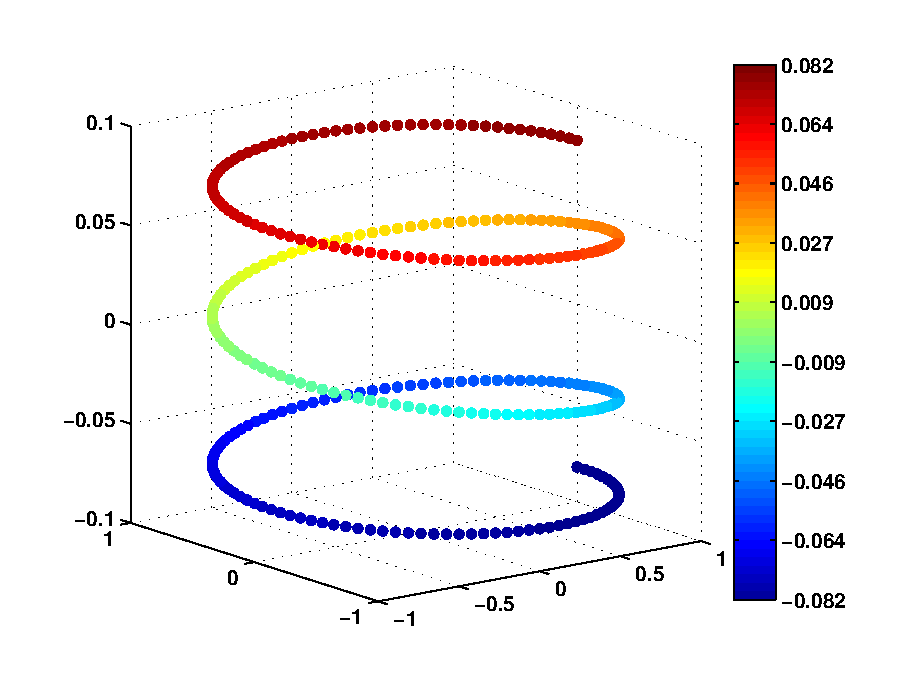
\includegraphics[width=0.45\textwidth]{helix.eps}}
\end{figure}
}

%\section{Error Accumulation}
%\subsection{analysis of error accumulation}
%\framee{Why Error Accumulation matters?}{
%\begin{block}{}
%\bc small errors + iterative(sequential) algorithm = \textbf{error accumulation} \ec
%\end{block}
%A simple example in computational mathematics: \\
%Define
%\be doubling(x)=\left\{
%\ba{ll}
%2x  & 0\leq x \leq 1/2 \\
%2x-1 & 1/2<x\leq 1 \\ \ea
%\right. \ee
%Iterate: $x_{k+1} = doubling(x_k)$. If starts at $x_0=0.4$, it should cycle in this way: $0.4\rightarrow 0.8\rightarrow 0.6 \rightarrow 0.2 \rightarrow 0.4\rightarrow \cdots$  However,
%\begin{figure}
%  \centering
%  \subfigure{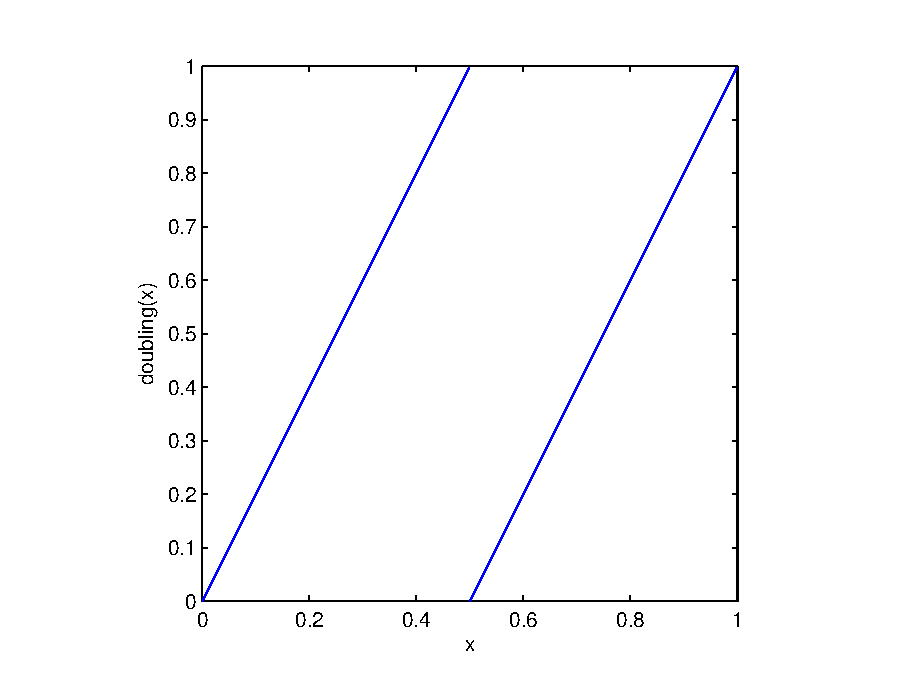
\includegraphics[width=0.45\textwidth]{doubling.eps}}
%  \subfigure{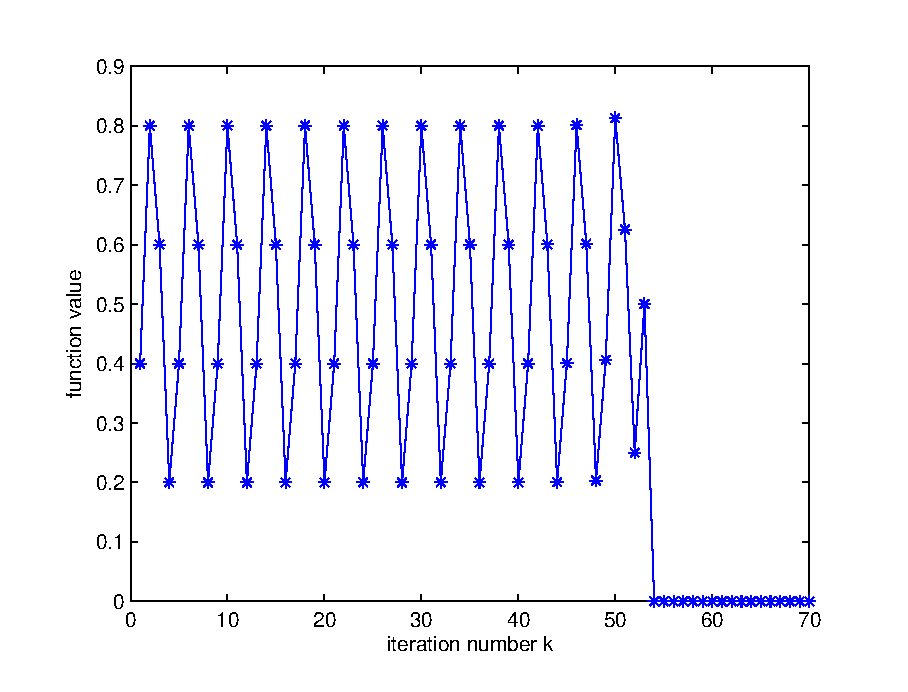
\includegraphics[width=0.45\textwidth]{doublingIter.eps}}
%  \caption{small round errors destroy a simple iteration}
%\end{figure}
%}
%
%\framee{Error Accumulation in Geometric GBA}{
%\begin{itemize}
%  \item now we analysis the case: exact distances + linear least square
%  \item point $j$ is to be determined, which has $l$ distances to the determined points $1,2,\ldots,l$, the computed coordinates are $x_i$, assume the ground truth are $\widehat{x}_i$, denote location error of point $i$ by $\delta x_i=x_i-\widehat{x}_i$ and assume $\delta x_i=O(\delta x)$
%  \item we need solve $\min_{x_j} \|Ax_j-b\|$, where
%  \be A = -2[x_{i+1}-x_i],\quad b=[(d_{i+1,j}^2-d_{ij}^2)-(\|x_{i+1}\|^2-\|x_i\|^2)]\ee
%  then we have
%  \begin{align}
%  \|x_{i+1}\|^2-\|x_i\|^2 & = \|\widehat{x}_{i+1}+\delta x_{i+1}\|^2-\|\widehat{x}_i+\delta x_i\|^2    \\
%   & = \|\widehat{x}_{i+1}\|^2-\|\widehat{x}_i\|^2 + 2\widehat{x}_{i+1}\delta x_{i+1} - 2\widehat{x}_i\delta x_i + \delta x_{i+1}^2-\delta x_i^2
%  \end{align}
%  therefore, $A=\widehat{A}+O(\delta x),~~b=\widehat{b}+O(\delta x)$
%  \begin{align}
%  \|Ax_j-b\| & =\|(\widehat{A}+\delta A)(\widehat{x}_j+\delta x_j)-(\widehat{b} + \delta b)\| \\
%   & =\|\widehat{A}\widehat{x}-\widehat{b}+\widehat{A} \delta x_j - O(\delta x)\|
%  \end{align}
%  \vskip-3mm
%
%  \item error in each step comes from
%  \begin{itemize}
%    \item errors \textbf{inherit} from previous steps
%    \item computational error: round error and \textbf{ill-conditioned} coefficient matrix $A$
%  \end{itemize}
%\end{itemize}
%}
%
%\framee{a toy example}{
%\begin{figure}
%  \centering
%  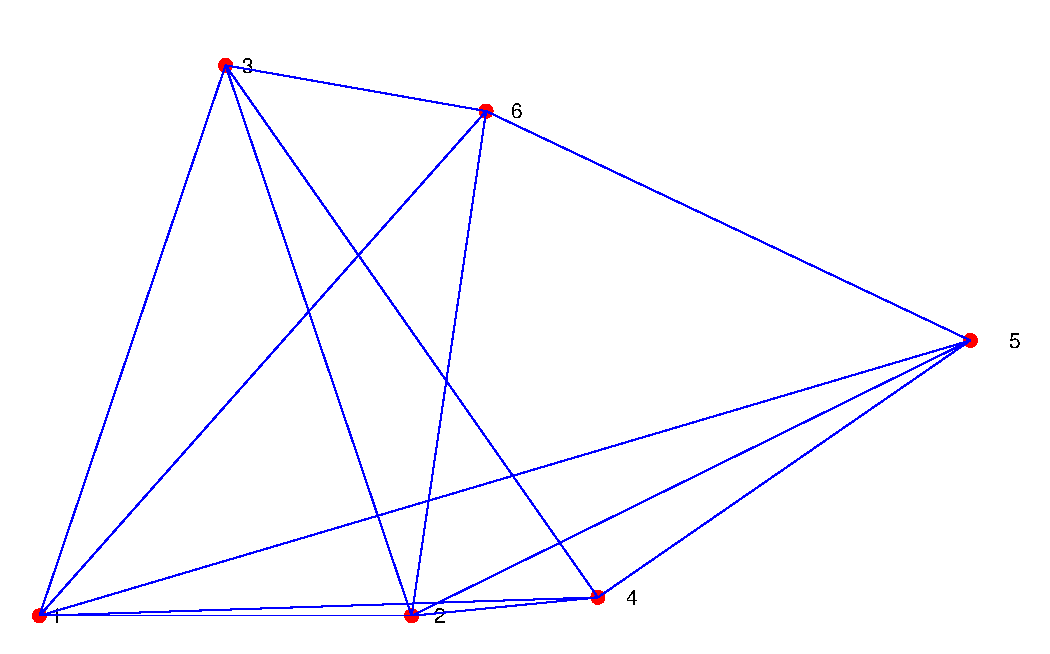
\includegraphics[width=0.8\textwidth]{toyEX1.eps}\\
%  \caption{a toy example to illustrate the importance of the computational order}
%\end{figure}
%}
%
%\subsection{our improvement}
%\framee{our improvement: specified computational order}{
%\begin{itemize}
%  \item We exploit two kinds of information to choose point $j$
%    \begin{itemize}
%     \item \textbf{structure information}: the largest number of known distances \\
%    Let $\mathcal{Y}$ be index set of determined points and $\mathcal{N} = \{1,2,\ldots,n\}\backslash \mathcal{Y}$ the undetermined ones, we define
%    \be p(i) = \sharp \{d_{ik}\neq 0 ~:~k\in \mathcal{Y}\}, ~~for~i\in \mathcal{N} \ee
%    and \be \mathcal{I} = \{i: p(i) = \max_{k\in \mathcal{N}} p(k)\} \ee
%    \item \textbf{distance information}: closest to the determined points \\
%    \be j = \arg\min_{i\in \mathcal{I}} \sum_{k\in \mathcal{Y}} d_{ik} \ee
%    \end{itemize}
%  \item Through this computational order
%    \begin{itemize}
%      \item remove oscillation -- "go far away and come back" [a movie]
%      \item utilize more distance information in total
%      \item almost always good-conditional $A$ $\rightarrow$ computational difficulty is avoided
%    \end{itemize}
%\end{itemize}
%}
%
%
%
%%\begin{figure}[ht]
%%      \includemovie[
%%        %poster,
%%        text={ (Animation of the computational order) }
%%      ]{2cm}{2cm}{sensor.avi}
%%\end{figure}
%
%\framee{another improvement: stress minimization}{
%\begin{itemize}
%  \item After computing $X_j$ by linear/nonlinear least square, we further
%    \be minimize ~~f(j,N(j)) \label{jNj}\ee
%    where $f$ is the stress function introduced before, to slightly adjust the locations of point $j$ and its neighbours, exploiting only the given distances among them.
%  \item benefits:
%    \begin{itemize}
%      \item only the given distances are involved in problem \reff{jNj}, no errors from previous calculation
%      \item problem \reff{jNj} is small-sized, not so much cost is added
%      \item least square solution can be viewed as a good initial point for this "difficult" problem
%    \end{itemize}
%\end{itemize}
%}
%
%\framee{Numerical results}{
%\setlength{\tabcolsep}{3pt}
%\begin{table}
%\begin{tabular}{|crr|rrr|rr|rrr|}
%  \hline
%  ID   &  num & per  & \multicolumn{3}{c|}{degree} & \multicolumn{1}{c}{RMSD} & fval & \multicolumn{3}{c|}{time(s)}  \\
%  \cline{4-6 } \cline{9-11}
%       &      &      & max & min & ave &       &        &    before& post & total  \\
%  \hline
%  1PTQ &  402 & 8.79&61&  6 &35.3& 1.53e-01&   75.91 & 3.9 &   0.3&   4.2 \\
%  1HOE &  558 & 6.55&65& 11 &36.5& 1.02e-01&  107.14 & 5.8 &   0.4&   6.2 \\
%  1LFB &  641 & 5.57&59&  8 &35.7& 1.79e-01&  124.43 & 7.3 &   0.5&   7.8 \\
%  1PHT &  811 & 5.37&75&  7 &43.5& 1.78e-01&  197.98 &10.6 &   0.7&  11.3 \\
%  1POA &  914 & 4.07&67&  8 &37.2& 1.64e-01&  181.64 &11.3 &   0.8&  12.0 \\
%  1AX8 & 1003 & 3.74&59&  7 &37.5& 1.29e-01&  205.92 &10.5 &   0.9&  11.4 \\
%  1F39 & 1534 & 2.43&62&  7 &37.2& 1.80e-01&  310.26 &16.3 &   1.8&  18.1 \\
%  1RGS & 2015 & 1.87&66&  4 &37.7& 1.98e-01&  415.34 &22.3 &   2.6&  24.9 \\
%  1KDH & 2846 & 1.36&64&  5 &38.8& 1.73e-01&  608.00 &35.2 &   4.9&  40.0 \\
%  1BPM & 3671 & 1.12&64&  4 &40.9& 1.22e-01&  850.69 &51.9 &   6.7&  58.6 \\
%  1RHJ & 3740 & 1.10&61&  5 &41.2& 1.21e-01&  883.84 &53.7 &   6.9&  60.7 \\
%  1HQQ & 3944 & 1.00&64&  5 &39.5& 1.78e-01&  886.72 &53.6 &   6.6&  60.2 \\
%  1TOA & 4292 & 0.94&62&  4 &40.1& 1.79e-01&  969.63 &61.8 &   7.4&  69.2 \\
%  1MQQ & 5681 & 0.75&66&  7 &42.4& 1.17e-01& 1373.82 &92.6 &  12.0& 104.7 \\
%  \hline
%\end{tabular}
%\caption{cutoff=6\AA, noise=5\%} \end{table}
%}

%\section{Laplacian Eigenmap}
\section{Laplacian matrix}
\framee{Laplacian matrix}{
\begin{block}{Definition: Laplacian matrix}
Given a graph $G=(V,E)$ and the parameter $t$, the Laplacian matrix $L$ is defined by $L=D-W$, where
    \be \omega_{ij} = \left \{
    \begin{array}{ll}
    exp(-\|x_i-x_j\|^2/t)  & if~ (i,j)\in E \\
    0                     & otherwise
    \end{array}
    \right.\ee
    and $D$ is a diagonal matrix with
    $$D_{ii}=\sum\nolimits_{j\neq i} \omega_{ij}.$$
\end{block}
\be L_{ij}=\left\{\ba{ll} -\omega_{ij} & i\neq j \\ \sum_{k\neq i}\omega_{ik} & i=j\ea\right. \ee


\begin{itemize}
  \item Note that when $t=\infty$, $W$ degenerates to the adjacency matrix.
  \item Research about Laplacian matrix is called \textbf{spectral graph theory}\footnote{Chung, Fan RK. \emph{Spectral graph theory}. Vol. 92. American Mathematical Soc., 1997.}.
  \item Two normalized variations:
    \begin{itemize}
      \item $L_{sym}:=D^{-1/2}LD^{-1/2}=I-D^{-1/2}WD^{-1/2}$
      \item $L_{rw}:=D^{-1}L = I-D^{-1}W$
    \end{itemize}
\end{itemize}
}

\framee{Some properties of Laplacian matrix }{
\begin{block}{}
For a graph $G$ and its Laplacian matrix $L$ with eigenvalues $\lambda_0 \leq \lambda_1 \leq \cdots \leq \lambda_{n-1}$
\vskip-1mm
\begin{enumerate}%[(1)]
  \item For every vector $f\in \mathbb{R}^n$ we have
        \be f^TLf=\frac{1}{2}\sum_{i,j=1}^n\omega_{ij}(f_i-f_j)^2 \ee
  \item L is symmetric and positive-semidefinite.
  \item $\lambda_0$ is always 0 because every Laplacian matrix has an eigenvector $v_0=[1,1,\dots,1]^T$.
  \item The number of times 0 appears as an eigenvalue in the Laplacian is the number of connected components in the graph.
\end{enumerate}
\end{block}
Proof of (1):
\begin{align*}
f^TLF & =f^TDf-f^TWf=\sum_{i=1}^nd_{ii}f_i^2-\sum_{i,j=1}^nf_if_j\omega_{ij}\\
 & =\frac{1}{2}\Big(\sum_{i=1}^nd_{ii}f_i^2-2\sum_{i,j=1}^nf_if_j\omega_{ij}+\sum_{j=1}^nd_{jj}f_j^2\Big)
 =\frac{1}{2}\sum_{i,j=1}^n\omega_{ij}(f_i-f_j)^2
\end{align*}
}

\section{Nonlinear dimensionality reduction}
\framee{Nonlinear dimensionality reduction}{
\begin{block}{Dimensionality Reduction Problem}
Given a set of $n$ points $x_1,\ldots, x_n$ in $\Real^l$, find a set of points $y_1,\ldots,y_n$ in $\Real^m (m\ll l)$ such that $y_i$ "represents" $x_i$.
\end{block}
Relation to DGP:\\
\begin{itemize}
  \item In noisy case, the distances can not be \textbf{precisely} realized in low-dimensional space.
  \item If the distances do not contradict with each other, the points can be precisely realized in high-dimensional space.
  \item a two-dimensional example
\end{itemize}
}



\framee{Optimal embedding}{
\begin{block}{}
Problem: Map the weighted graph $G$ to a line such that the adjacent vertices stay as close as possible.
\end{block}
Let $y=(y_1,y_2,\ldots,y_n)^T$ be such a map, so we want to minimize
\be \sum_{(i,j) \in E}(y_i-y_j)^2\omega_{ij}=y^TLy \ee
Therefore,
\be \min_{y^TDy=1,y^TDe=0} y^TLy \ee
gives us a reasonable solution.

\vskip2mm
\begin{block}{}
General case: Embed the graph into $m$-dimensional Euclidean space.
\end{block}
Let $Y=[y_1 ~y_2~\ldots ~ y_n]^T\in \Real^{n\times m}$ that each row gives a coordinate. Similarity we need to minimize
\be \sum_{(i,j)\in E} \|y_i-y_j\|^2\omega_{ij} = tr(Y^TLY) \ee
}

\framee{Courant-Fischer Theorem}{
\begin{block}{Courant-Fischer Theorem}
Let $A$ be a symmetric $n\times n$ matrix with eigenvalues $\lambda_1 \leq \lambda_2 \leq \ldots \leq \lambda_n$ and corresponding eigenvectors $v_1,v_2,\ldots,v_n$. For $1\leq k \leq n$, let $S_k$ denote the span of $v_1,\ldots,v_k$ (with $S_0=\{0\}$), and let $S_k^{\bot}$ denote the orthogonal complement of $S_k$. Then
$$\lambda_k = \min_{\|x\|=1,x\in S_{k-1}^{\bot}} x^TAx = \min_{x\in S_{k-1}^{\bot}} \frac{x^TAx}{x^Tx}$$
\end{block}
}

\framee{Nonlinear dimensionality reduction algorithm}{
\begin{block}{Nonlinear dimensionality reduction algorithm framework  ({\footnotesize Belkin-Niyogi, 2002})}
\begin{enumerate}[Step 1]
  \item Constructing the adjacency graph \\ (a) $\epsilon$-neighborhood \quad (b) $k$-nearest neighbors
  \item Choosing the weights \\ (a) Heat kernel \quad \quad ~~(b) Simple-minded
  \item Eigenmaps: $x_i\rightarrow (f_1(i),\ldots,f_m(i))$, where $Lf_i=\lambda_i Df_i$,\\ $0=\lambda_0 \leq \lambda_1 \leq \ldots \leq \lambda_{n-1}$.
\end{enumerate}
\end{block}
}

\framee{Grid points example 1}{
\begin{figure}
  \centering
  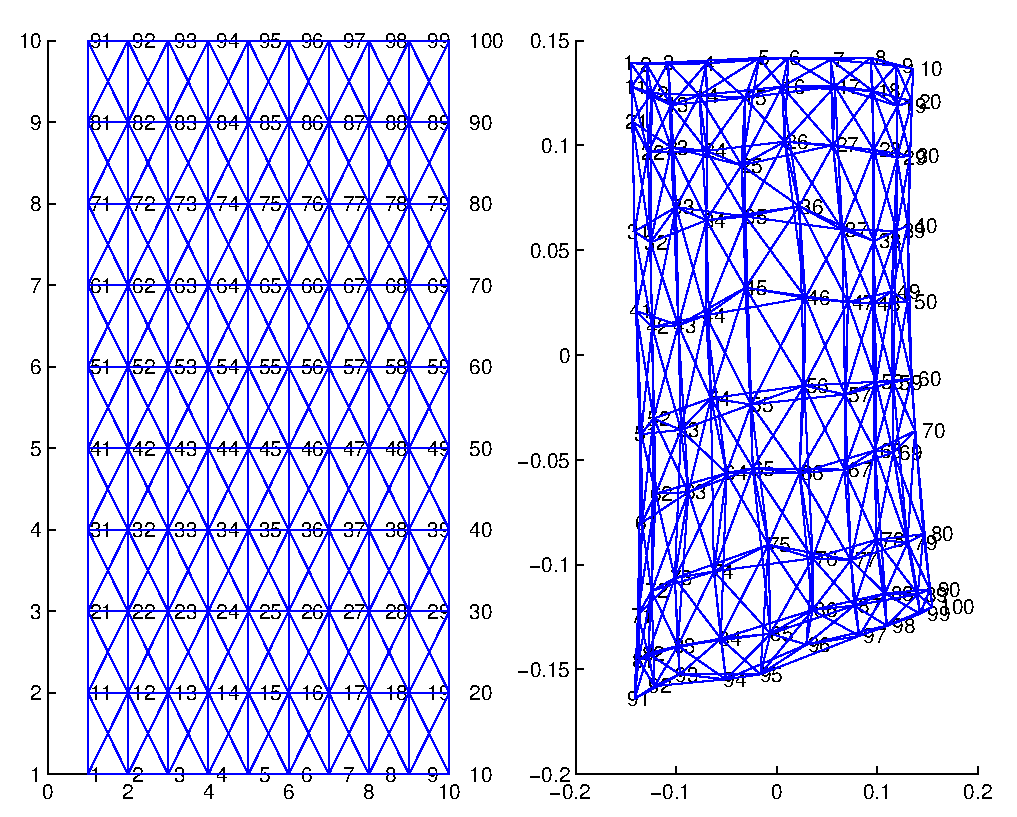
\includegraphics[width=0.85\textwidth]{5.eps}\\
  \caption{cutoff=2, degree: [12,5,10], noise = 20\%}
\end{figure}
}

\framee{Grid points example 2}{
\begin{figure}
  \centering
  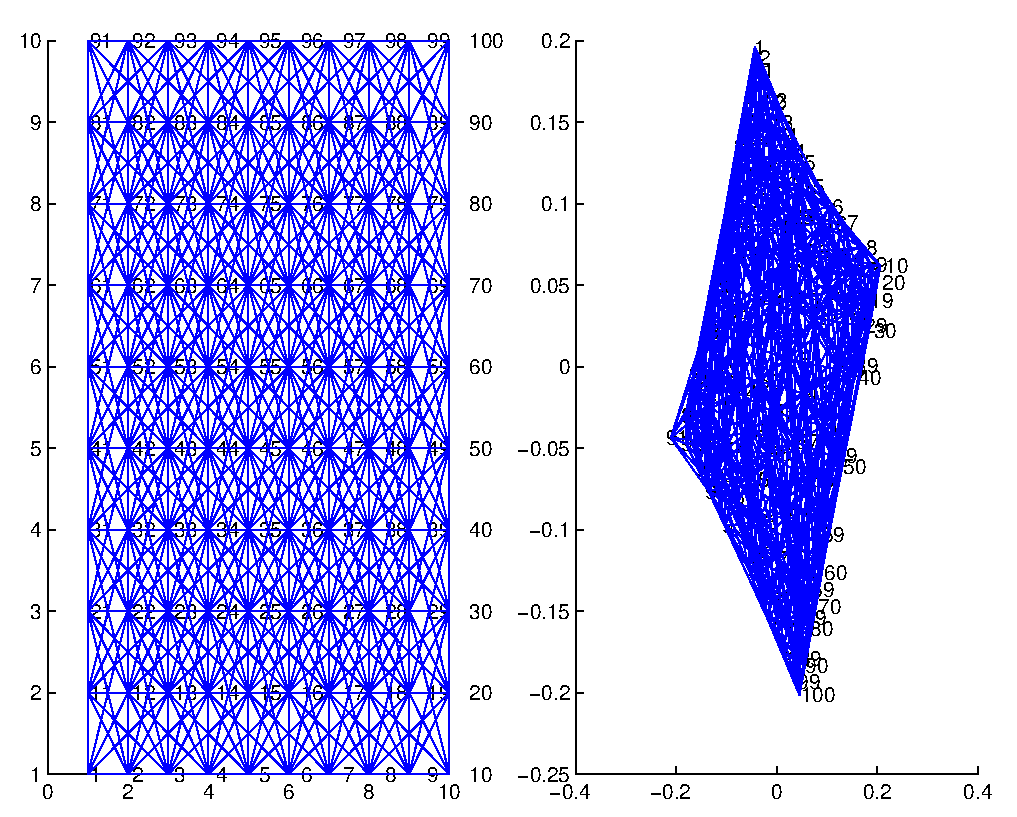
\includegraphics[width=0.85\textwidth]{6.eps}\\
  \caption{cutoff=3, degree: [20,10,21.2], noise = 20\%}
\end{figure}
}

\framee{a random example}{
\begin{figure}
  \centering
  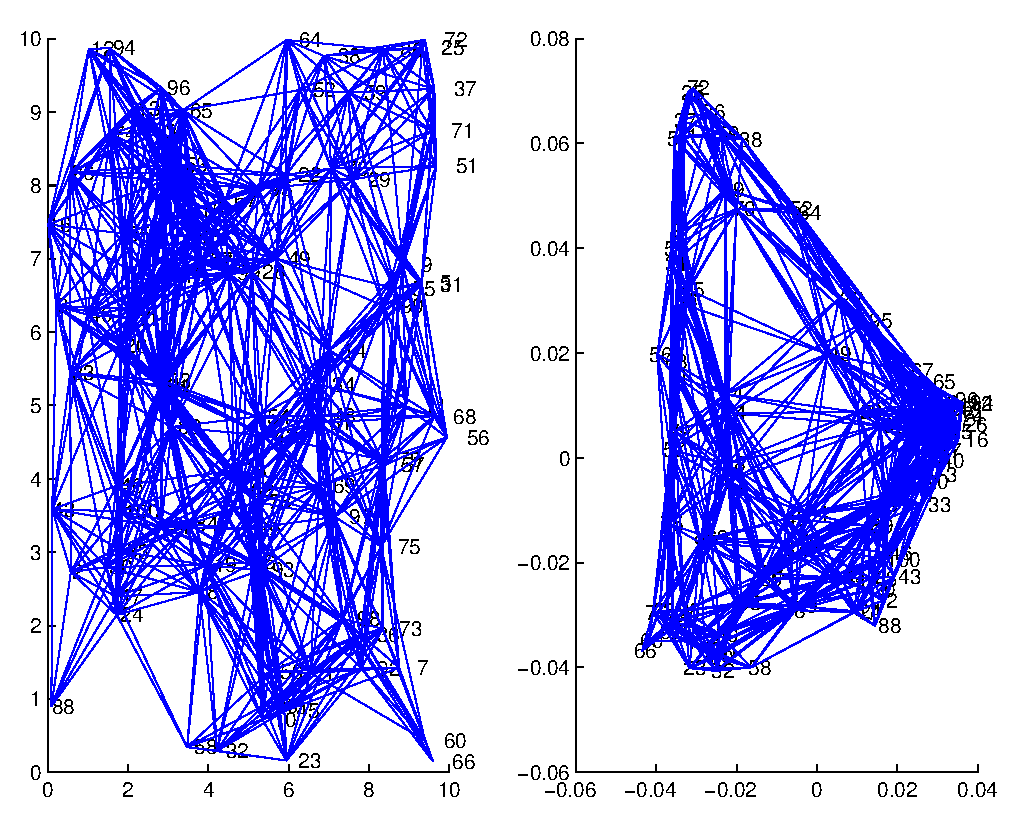
\includegraphics[width=0.85\textwidth]{7.eps}\\
\end{figure}
}

\framee{another random example}{
\begin{figure}
  \centering
  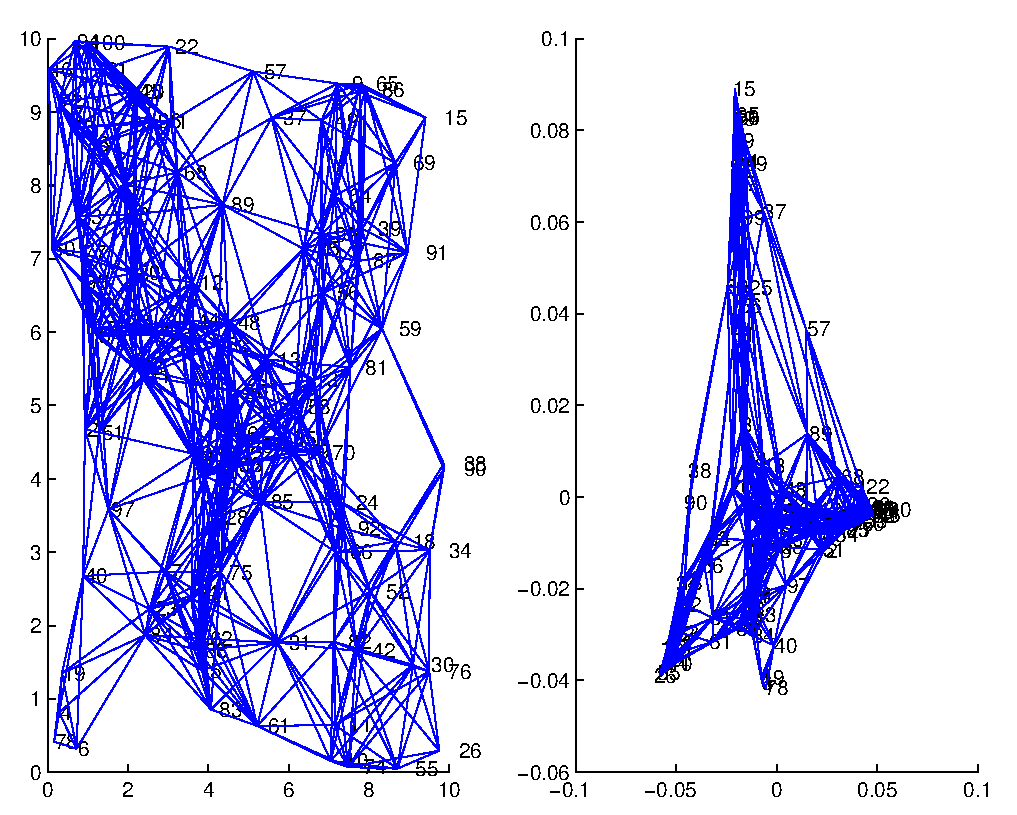
\includegraphics[width=0.85\textwidth]{8.eps}\\
\end{figure}
}

\framee{Remarks about Laplacian eigenmap}{
\begin{itemize}
  \item Accurate locations can not be recovered directly.
  \item Useful relative relation can be inferred.
  \item Balanced graph are preferred.
\end{itemize}
}

\section{Laplacian eigenmap-based localization algorithm}
\framee{Laplacian eigenmap-based localization algorithm }{
\begin{block}{Laplacian Eigenmap-based Localization Algorithm for DGP}
\begin{enumerate}[Step 1]
  \item Construct the Laplacian matrix $L$ and calculate its eigenvalue decomposition $L=VDV^T$ such that the eigenvalues in $D$ are in ascending order.
  \item Set $X0 = V(:,2:m+1)$ and scale it to the proper magnitude.
  \item Using $X0$ as the initial point, apply error function minimization method to further improve the result.
\end{enumerate}
\end{block}

\begin{block}{Scaling method}
\begin{enumerate}
  \item Construct a new distance matrix $\tilde{D}$ according to $X0$ and $E$.
  \item Calculate
      $$ratio = \frac{sum(D)}{sum(\tilde{D})}.$$
  \item Set $X0 = X0*ratio$.
\end{enumerate}
\end{block}
}

\framee{Random example}{
\begin{figure}
  \centering
  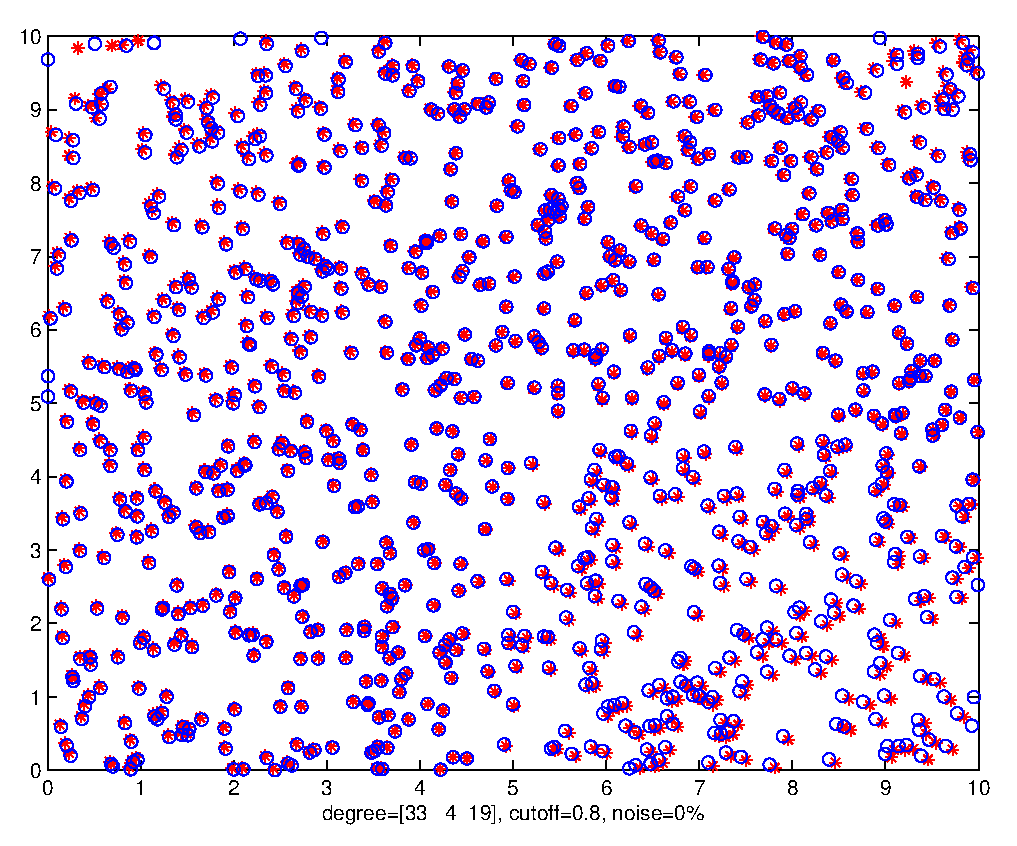
\includegraphics[width=0.8\textwidth]{test1.eps}\\
  %\caption{cutoff = 3, noise = 0}
\end{figure}
}

\framee{Random example}{
\begin{figure}
  \centering
  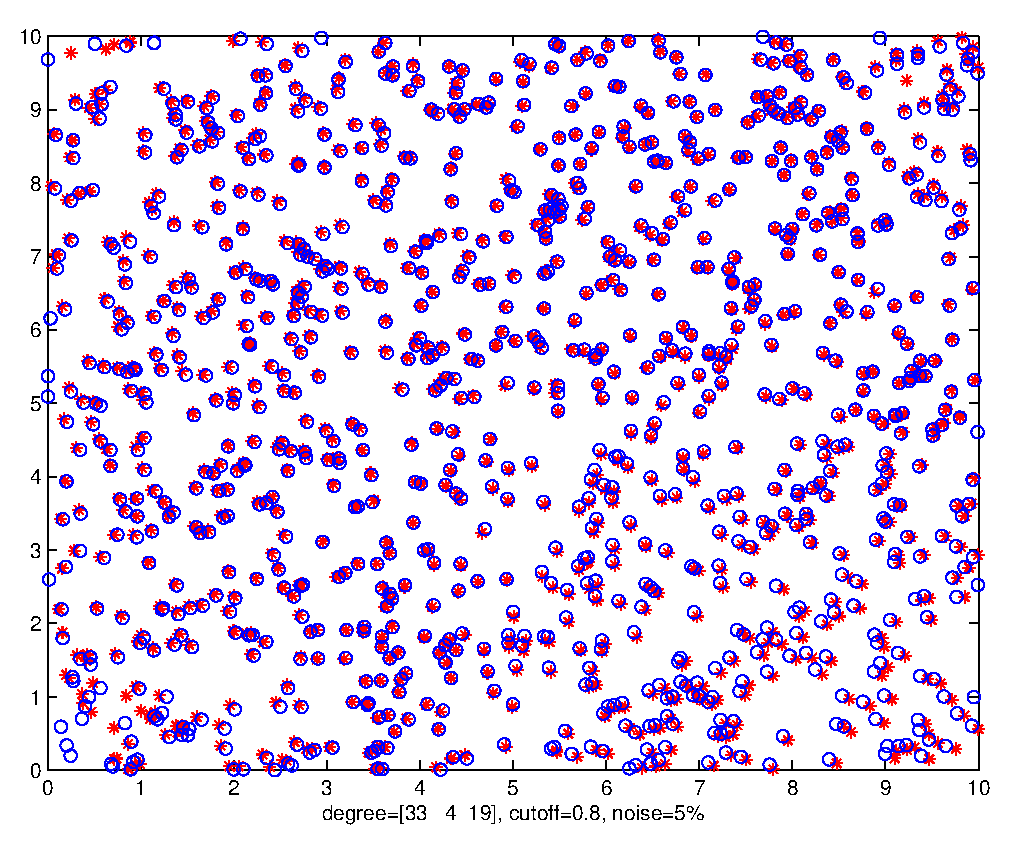
\includegraphics[width=0.8\textwidth]{test2.eps}\\
  %\caption{cutoff = 3, noise = 0}
\end{figure}
}

\framee{}{
\begin{figure}
  \centering
  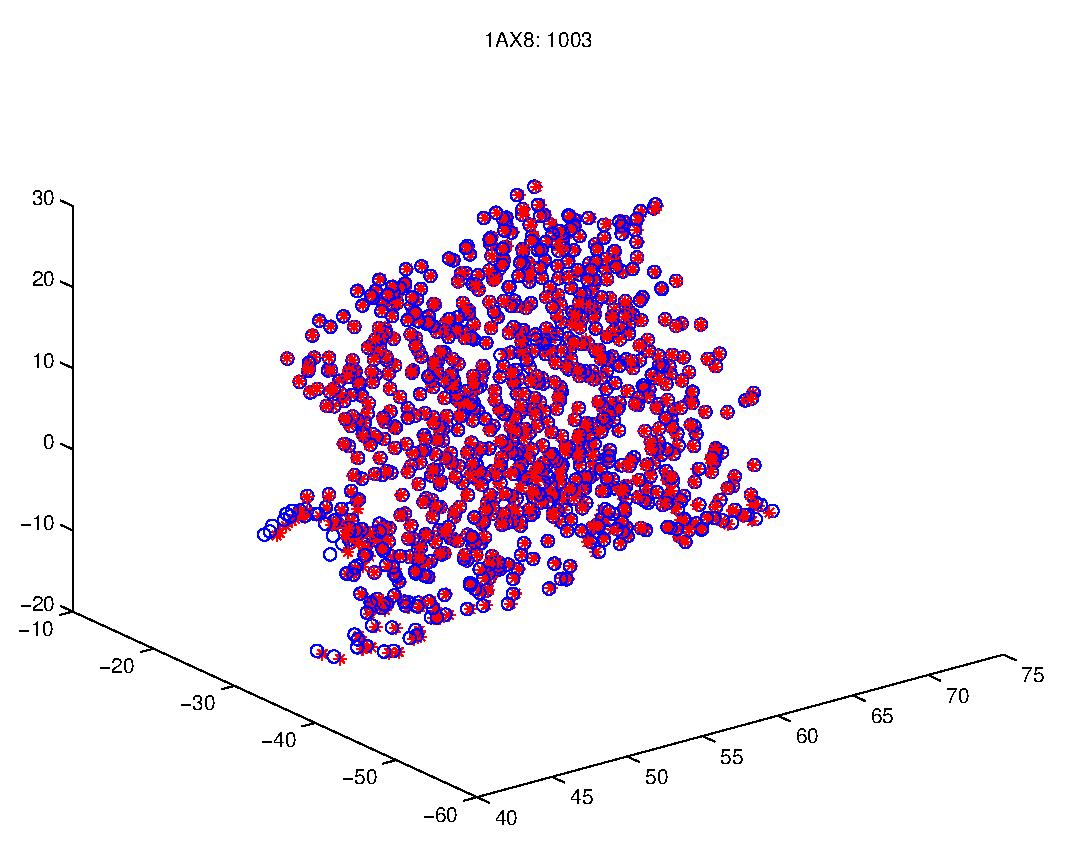
\includegraphics[width=1\textwidth]{1AX8.eps}\\
  %\caption{cutoff = 3, noise = 0}
\end{figure}
}

\framee{}{
\begin{figure}
  \centering
  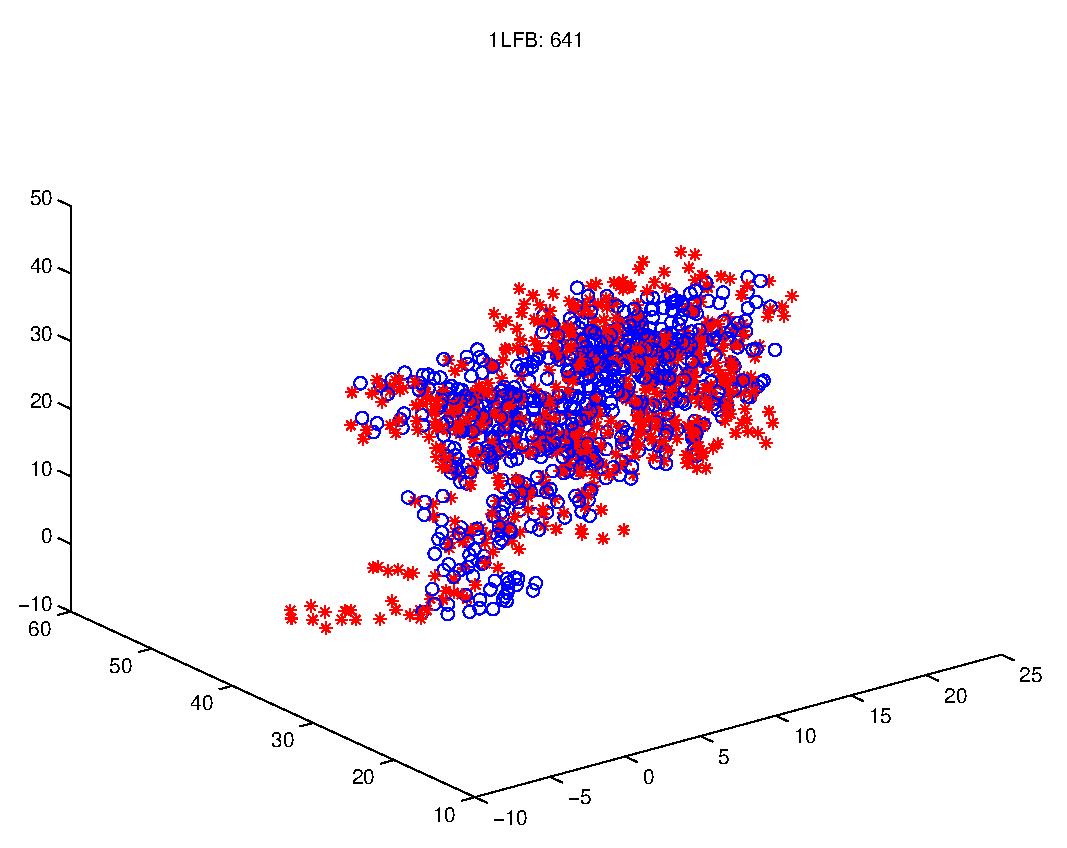
\includegraphics[width=\textwidth]{1LFB.eps}\\
  %\caption{cutoff = 3, noise = 0}
\end{figure}
}

\framee{Discussions}{
\begin{itemize}
  \item Pros
    \begin{itemize}
      \item very simple and fast
      \item relatively robust to the noise
      \item good in uniformly generated random instances
    \end{itemize}
  \item Cons
    \begin{itemize}
      \item sensitive to the parameter $t$ and no theoretically-guaranteed good way to choose it
      \item terrible in most of real protein instances, except for 1PTQ, 1HOE, 1AX8
    \end{itemize}
\end{itemize}
}

\framee{possible distributed algorithm}{
\begin{figure}
  \centering
  \subfigure{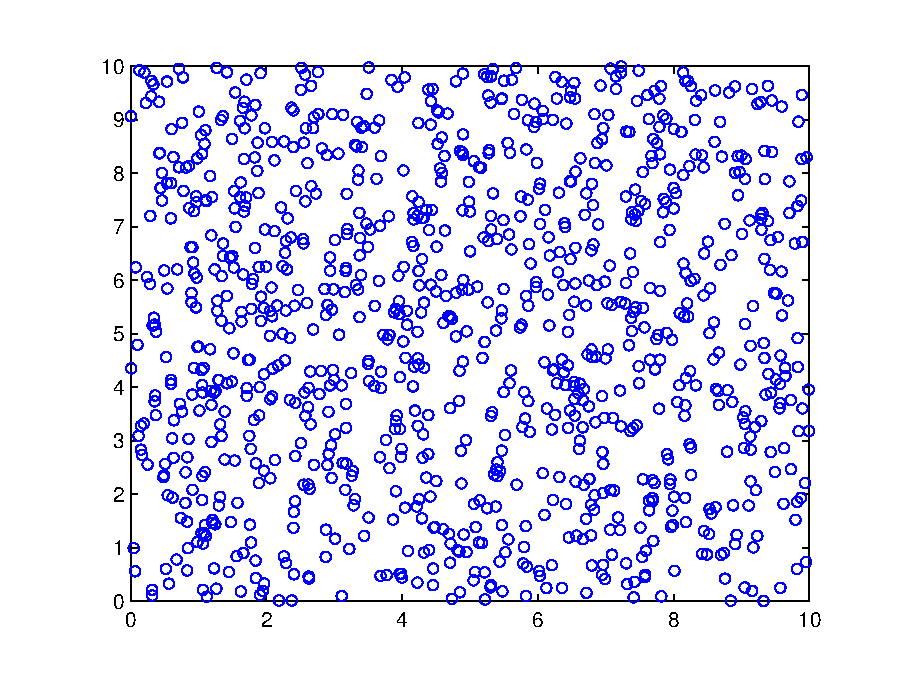
\includegraphics[width=0.45\textwidth]{Original.eps}}\\
  \subfigure{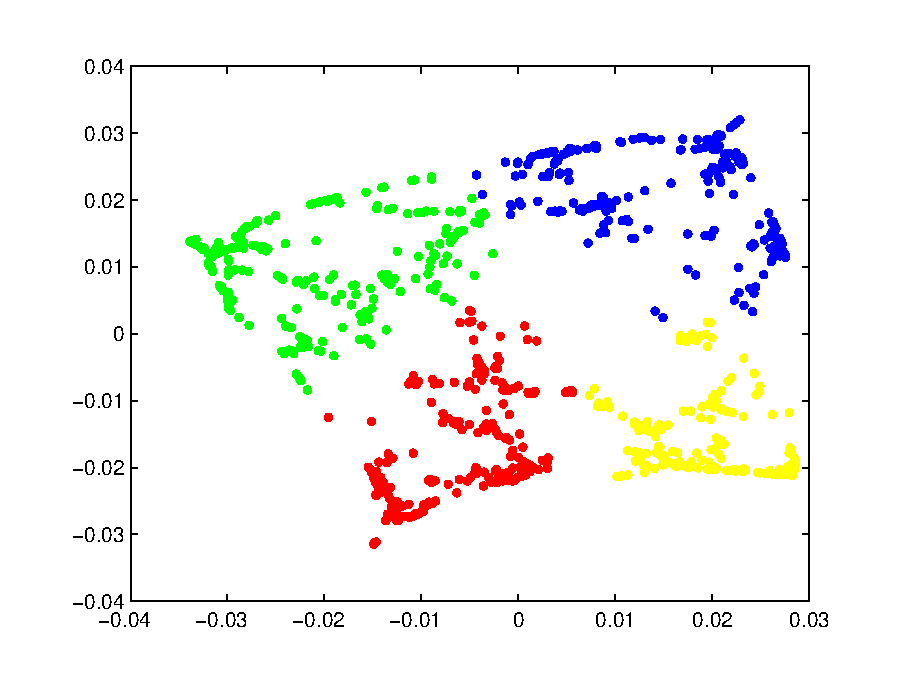
\includegraphics[width=0.45\textwidth]{ClusterV.eps}}
  \subfigure{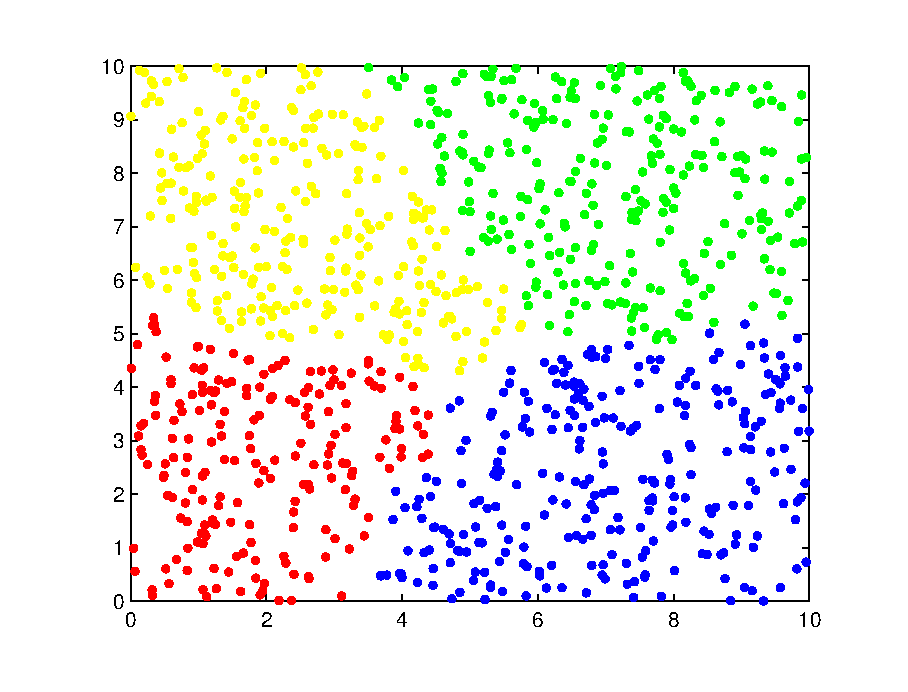
\includegraphics[width=0.45\textwidth]{ClusterX.eps}}
\end{figure}
}


%\section{possible Laplacian-based Distributed Algorithm }
%\framee{Spectral Clustering}{
%\begin{figure}
%  \centering
%  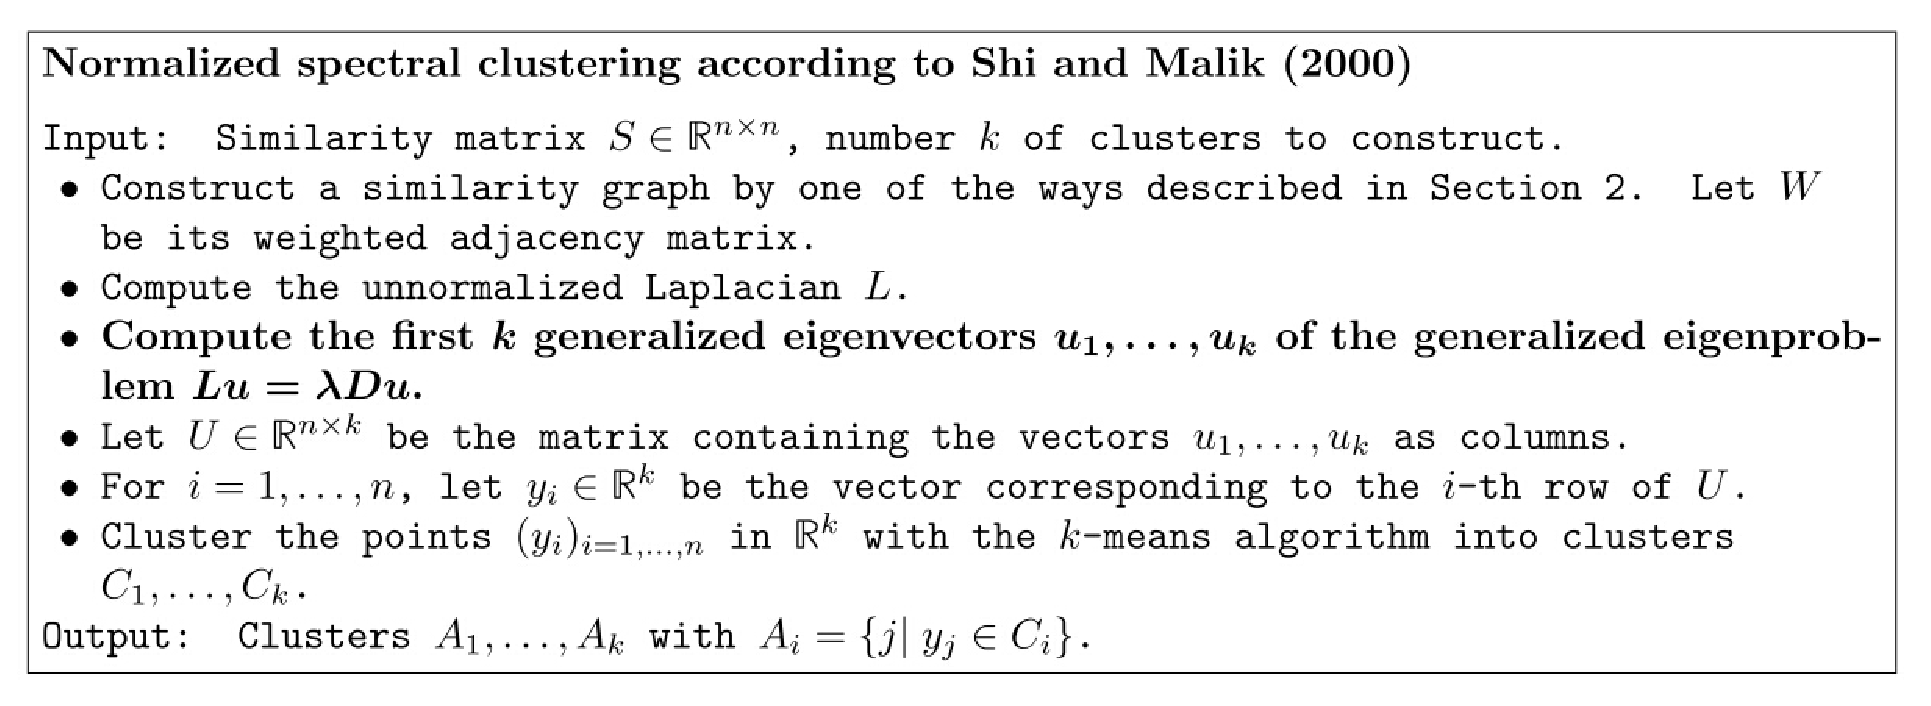
\includegraphics[width=\textwidth]{clusterAlgo.eps}\\
%  %\caption{cutoff = 3, noise = 0}
%\end{figure}
%}
%
%\framee{Remarks about Spectral Clustering for DGP}{
%{\large
%\begin{itemize}
%  \item good news: clusters have been observed in numerical results
%  \vskip3mm
%  \item main difficulties:
%    \begin{itemize}
%      \item no obvious clusters exist in proteins
%      \item hard to choose the prescribed cluster number $k$
%      \item stable stitch step need reliable \textbf{overlapping points}
%    \end{itemize}
%\end{itemize}
%}
%}

%\section{Stress Majorization}
%\subsection{Principle of Majorization}
%\framee{Principle of Majorization\footnote{Borg, Ingwer, and Patrick JF Groenen. \emph{Modern multidimensional scaling: Theory and applications}. Springer, 2005.}}{
%\begin{itemize}
%  \item The central idea of the majorization method is to replace iteratively the original complicated function $f(x)$ by an auxiliary function $g(x,z)$, where $z$ in $g(x,z)$ is some fixed value.
%      \vskip2mm
%  \item $g(x,z)$ is a \emph{majorization function} of $f(x)$ if it satisfies
%    \begin{itemize}
%     \item $g(x,z)$ should be simpler to minimize than $f(x)$.
%     \item the original function must always be smaller than or at most equal to the auxiliary function, i.e., $f(x)\leq g(x,z)$.
%    \item the auxiliary function should touch the surface at the so-called \emph{supporting point} $z$, i.e., $f(z)=g(z,z)$.
%    \end{itemize}
%    \begin{figure}
%  \centering
%  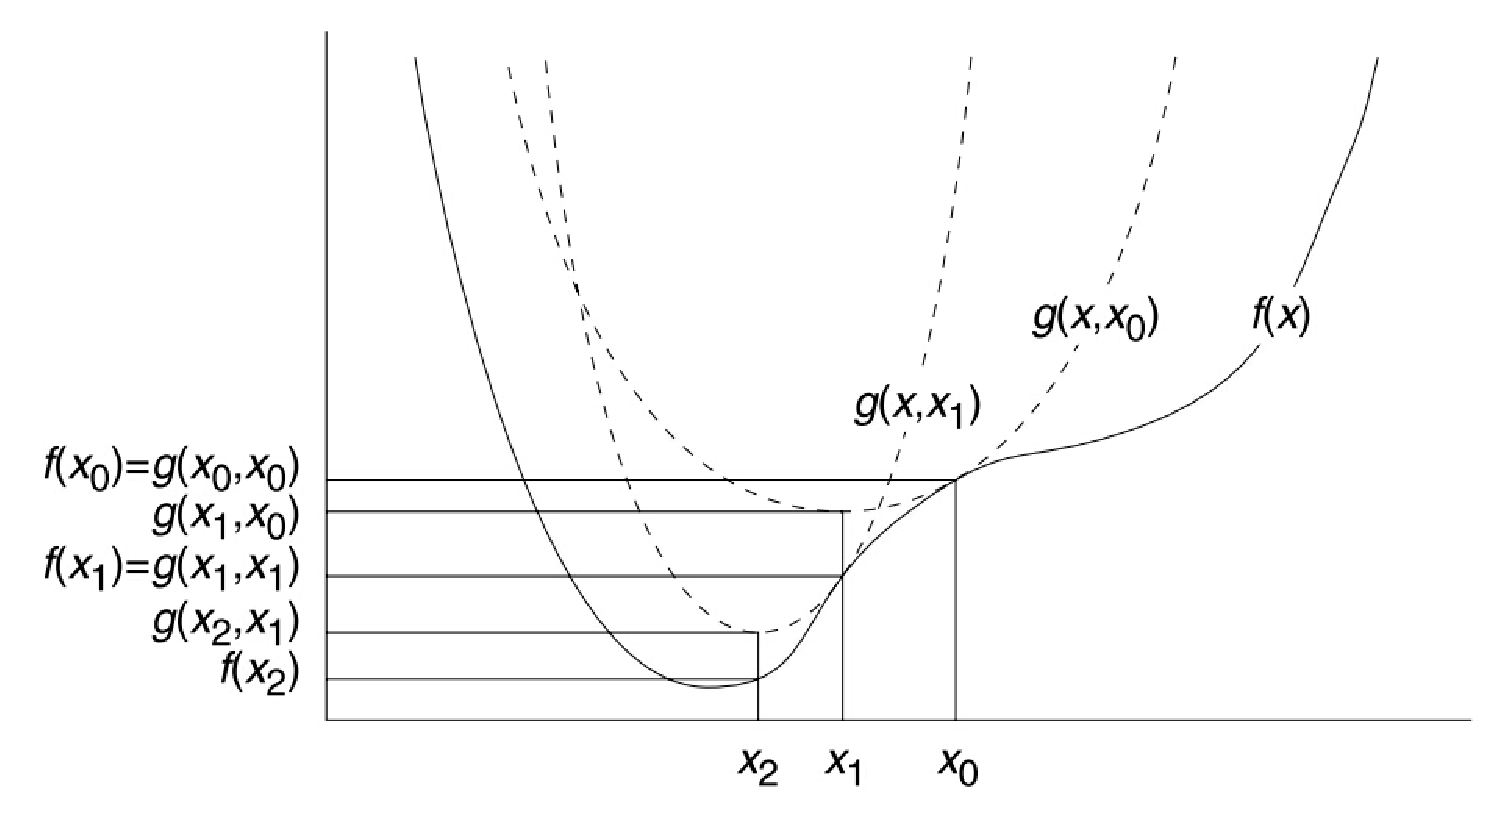
\includegraphics[width=0.6\textwidth]{majorization.eps}\\
%  %\caption{Illustration of two iterations of the iterative majorization method }
%\end{figure}
%  \item \emph{monotone decreasing}: let $x^*=\arg\min_x g(x,z)$, then we have
%  \be f(x^*)\leq g(x^*,z)\leq g(z,z)=f(z) \ee
%\end{itemize}
%}
%
%\subsection{Stress Majorization}
%\framee{Stress Majorization(1)}{
%\begin{itemize}
%  \item A widely used technique in Multidimensional Scaling (MDS) community.
%  \item MDS is a means of visualizing the level of similarity of individual cases of a dataset.
%      %It refers to a set of related ordination techniques used in information visualization, in particular to display the information contained in a distance matrix.
%      An MDS algorithm aims to place each object in $N$-dimensional space such that the between-object distances are preserved as well as possible\footnote{http://en.wikipedia.org/wiki/Multidimensional\_scaling}.
%  \item Let $X=(x_1,x_2,\ldots,x_n)^T \in \mathbb{R}^{n\times r}$, where each row is the coordinate of one point, and each column denotes one axis, rewrite
%    \begin{align}
%        Stress(X) & =\sum_{i<j}\omega_{ij}(\|x_i-x_j\|-d_{ij})^2 \\
%          & =\sum_{i<j}\omega_{ij}d_{ij}^2 + \sum_{i<j}\omega_{ij}\|x_i-x_j\|^2 -2\sum_{i<j}\omega_{ij}d_{ij}\|x_i-x_j\|
%    \end{align}
%  \item The second term $\sum_{i<j}\omega_{ij}\|x_i-x_j\|^2 =Tr(X^TL^{\omega}X)$, where
%    \be L_{ij}^{\omega}=\left\{\ba{ll} -\omega_{ij} & i\neq j \\ \sum_{k\neq i}\omega_{ik} & i=j\ea\right. \ee
%\end{itemize}
%}
%
%\framee{Stress Majorization(2)}{
%\begin{itemize}
%  \item Now we bound the third term. By Cauchy-Schwartz inequality,
%    \be (x_i-x_j)^T(z_i-z_j)\leq \|x_i-x_j\|\|z_i-z_j\| \ee
%    then we have
%    \be  \sum_{i<j}\omega_{ij}d_{ij}\|x_i-x_j\|\geq \sum_{i<j}\omega_{ij}d_{ij}inv(\|z_i-z_j\|)((x_i-x_j)^T(z_i-z_j)) = Tr(X^TL^ZZ) \ee
%    where $inv(x)=1/x$ when $x\neq 0$ and 0 otherwise, and
%    \be L_{ij}^Z=\left\{\ba{ll} -\omega_{ij}d_{ij}inv(\|z_i-z_j\|) & i\neq j \\ -\sum_{j\neq i}L_{ij}^Z & i=j\ea\right. \ee
%  \item In summary, $Stress(X)$ can be bounded by $F^Z(X)$ defined as
%  \be F^Z(X) = \sum_{i<j}\omega_{ij}d_{ij}^2 +Tr(X^TL^{\omega}X)-2Tr(X^TL^ZZ)\ee
%  \item The minima of $F^Z(X)$ are given by solving
%  \be L^{\omega}X=L^ZZ \ee
%  \item the algorithm converges to a stationary point linearly.
%\end{itemize}
%}



\section{Conclusion and Future Work}
\frame{
\frametitle{Conclusion and Future Work}
\begin{itemize}
\item Conclusion
    \begin{itemize}
        \item Proposed a Laplacian Eigenmap-based algorithm for DGP, which is a totally new idea for solving this NP-hard problem.
        \item Finished some preliminary numerical experiments to show its efficiency.
    \end{itemize}
\item Future Work
    \begin{itemize}
      \item Figure out the problem with protein computation.
      \item Carefully study the parameters in Laplacian matrix.
     % \item Eliminate some edges to reduce the computational complexity in nonlinear programming.
      \item Develop distributed algorithm based Laplacian Eigenmap.
    \end{itemize}
\end{itemize}
}


\frame{
%\frametitle{Q \& A}
\begin{center}
  \Large{  \textsc{Thank you for your attention!}}  \\
  \vspace{0.2cm}
  {\blue szl@lsec.cc.ac.cn }
\end{center}
}

\end{CJK*}
\end{document}
